% Generated 2021-02-06 01:28:14 +0530
\subsection{Specifications} \label{sec:Specifications}


This section provides semantic information for the \block{Specifications} model.

\begin{figure}[ht]
  \centering
    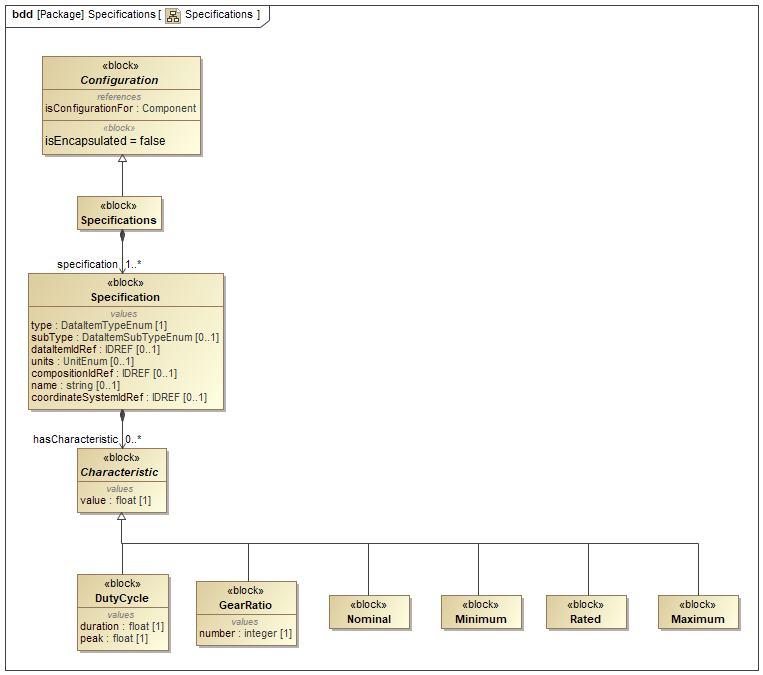
\includegraphics[width=1.0\textwidth]{figures/Specifications.png}
  \caption{Specifications Diagram}
  \label{fig:Specifications Diagram}
\end{figure}

\FloatBarrier


Note: See \fig{Specifications Schema Diagram} for XML schema.


\subsubsection{Specifications}




\block{Specifications} \glspl{organize} \block{Specification} elements for a \block{Component}.


\paragraph{Elements of Specifications}\mbox{}
\label{sec:Elements of Specifications}

\tbl{Elements of Specifications} lists the elements of \texttt{Specifications}.

\begin{table}[ht]
\centering 
  \caption{Elements of Specifications}
  \label{table:Elements of Specifications}
\tabulinesep=3pt
\begin{tabu} to 6in {|l|l|} \everyrow{\hline}
\hline
\rowfont\bfseries {Element} & {Multiplicity} \\
\tabucline[1.5pt]{}
\texttt{Specification} & 1..* \\
\end{tabu}
\end{table}
\FloatBarrier


Descriptions for elements of \block{Specifications}:

\begin{itemize}

\item \block{Specification} \newline \block{Specification} elements define information describing the design characteristics for a piece of equipment.

\end{itemize}



\subsubsection{Specification}
\label{sec:Specification}



\block{Specification} elements define information describing the design characteristics for a piece of equipment.



\paragraph{Attributes of Specification}\mbox{}
\label{sec:Attributes of Specification}

\tbl{Attributes of Specification} lists the attributes of \texttt{Specification}.

\begin{table}[ht]
\centering 
  \caption{Attributes of Specification}
  \label{table:Attributes of Specification}
\tabulinesep=3pt
\begin{tabu} to 6in {|l|l|l|} \everyrow{\hline}
\hline
\rowfont\bfseries {Attribute} & {Type} & {Multiplicity} \\
\tabucline[1.5pt]{}

\property{type}[Specification] & \texttt{DataItemTypeEnum} & 1 \\
\property{subType}[Specification] & \texttt{DataItemSubTypeEnum} & 0..1 \\
\property{dataItemIdRef}[Specification] & \texttt{IDREF} & 0..1 \\
\property{units}[Specification] & \texttt{UnitEnum} & 0..1 \\
\property{compositionIdRef}[Specification] & \texttt{IDREF} & 0..1 \\
\property{name}[Specification] & \texttt{string} & 0..1 \\
\property{coordinateSystemIdRef}[Specification] & \texttt{IDREF} & 0..1 \\
\property{id}[Specification] & \texttt{ID} & 0..1 \\
\property{originator}[Specification] & \texttt{OriginatorEnum} & 0..1 \\
\end{tabu}
\end{table}
\FloatBarrier

Descriptions for attributes of \block{Specification}:

\begin{itemize}

\item \property{type}[Specification] \newline Same as \block{DataItem} type. See \sect{DataItem Types}.

\item \property{subType}[Specification] \newline Same as \block{DataItem} subtypes. See \sect{DataItem SubTypes}.

\item \property{dataItemIdRef}[Specification] \newline A reference to the \property{id} attribute of the \block{DataItem} associated with this element.

\item \property{units}[Specification] \newline Same as \block{DataItem} units. See \sect{DataItem}.

\item \property{compositionIdRef}[Specification] \newline A reference to the \property{id} attribute of the \block{Composition} associated with this element.

\item \property{name}[Specification] \newline The \property{name} provides additional meaning and differentiates between \block{Specifications}.

\item \property{coordinateSystemIdRef}[Specification] \newline References the \block{CoordinateSystem} for geometric \block{Specification} elements.

\item \property{id}[Specification] \newline The unique identifier for this \block{Specification}.

The \property{id} attribute \textbf{MUST} be unique within the \gls{MTConnectDevices Response Document}.

\item \property{originator}[Specification] \newline A reference to the creator of the \block{Specification}.

\texttt{OriginatorEnum} Enumeration:

\begin{itemize}
\item \texttt{MANUFACTURER} \newline The manufacturer of a piece of equipment or \block{Component}. 
\item \texttt{USER} \newline The owner or implementer of a piece of equipment or \block{Component}. 
\end{itemize}

\end{itemize}


\paragraph{Elements of Specification}\mbox{}
\label{sec:Elements of Specification}

\tbl{Elements of Specification} lists the elements of \texttt{Specification}.

\begin{table}[ht]
\centering 
  \caption{Elements of Specification}
  \label{table:Elements of Specification}
\tabulinesep=3pt
\begin{tabu} to 6in {|l|l|} \everyrow{\hline}
\hline
\rowfont\bfseries {Element} & {Multiplicity} \\
\tabucline[1.5pt]{}
\texttt{Characteristic} & 0..* \\
\end{tabu}
\end{table}
\FloatBarrier


Descriptions for elements of \block{Specification}:

\begin{itemize}

\item \block{Characteristic} \newline \block{Characteristic} is an abstract element of \block{Specification}.
\end{itemize}



\subsubsection{ProcessSpecification}
\label{sec:ProcessSpecification}



\block{ProcessSpecification} provides information used to assess the conformance of a variable to process requirements.

See \sect{Limits for ProcessSpecification} for details on the \block{ProcessSpecification} model.


\paragraph{Elements of ProcessSpecification}\mbox{}
\label{sec:Elements of ProcessSpecification}

\tbl{Elements of ProcessSpecification} lists the elements of \texttt{ProcessSpecification}.

\begin{table}[ht]
\centering 
  \caption{Elements of ProcessSpecification}
  \label{table:Elements of ProcessSpecification}
\tabulinesep=3pt
\begin{tabu} to 6in {|l|l|} \everyrow{\hline}
\hline
\rowfont\bfseries {Element} & {Multiplicity} \\
\tabucline[1.5pt]{}
\texttt{Limits} & 0..* \\
\end{tabu}
\end{table}
\FloatBarrier


Descriptions for elements of \block{ProcessSpecification}:

\begin{itemize}

\item \block{Limits} \newline \block{Limits} is an abstract element of \block{ProcessSpecification} that represents a set of conformance boundaries or conditions for a variable.
\end{itemize}



\subsubsection{Characteristic}
\label{sec:Characteristic}



\block{Characteristic} is an abstract element of \block{Specification}.


The value of \texttt{Characteristic} \MUST be \texttt{float}.

The following sections define the types of \block{Characteristic}s.

\subsubsection{Maximum}
\label{sec:Maximum}



A numeric upper constraint.




\subsubsection{Minimum}
\label{sec:Minimum}



A numeric lower limit constraint.



\subsubsection{Nominal}
\label{sec:Nominal}



The numeric target or expected value.



\subsubsection{LowerLimit}
\label{sec:LowerLimit}



The lower conformance boundary for a variable.

Note to Entry: immediate concern or action may be required.



\subsubsection{LowerWarning}
\label{sec:LowerWarning}



The lower boundary indicating increased concern and supervision may be required.



\subsubsection{UpperLimit}
\label{sec:UpperLimit}



The upper conformance boundary for a variable.

Note to Entry: immediate concern or action may be required.




\subsubsection{UpperWarning}
\label{sec:UpperWarning}



The upper boundary indicating increased concern and supervision may be required.


